\documentclass[a4paper,10pt]{article}
\usepackage[margin=1in]{geometry}
\usepackage{amsmath,amsthm,amssymb,amsfonts,stmaryrd}
\usepackage{soul}
\usepackage{array}
\usepackage{empheq}
\usepackage{xfrac}
\usepackage{minibox}
\usepackage{enumitem}
	\setlist{nosep} % or \setlist{noitemsep} to leave space around whole list
\usepackage{color}
\usepackage{blkarray}
\setcounter{MaxMatrixCols}{20}
\usepackage{showlabels}
\usepackage{arydshln}	% Dotted lines in arrays
\usepackage{adjustbox}
\usepackage{hyperref}
\hypersetup{
  colorlinks   = true, %Colours links instead of ugly boxes
  urlcolor     = blue, %Colour for external hyperlinks
  linkcolor    = blue, %Colour of internal links
  citecolor   = red %Colour of citations
}
\usepackage{cleveref}
\usepackage{multirow}
\usepackage{comment}


\newtheorem{lemma}{Lemma}
\newtheorem{definition}{Definition}
\newtheorem{theorem}{Theorem}
\newtheorem{corollary}{Corollary}
\newtheorem{assumption}{Assumption}

\newcommand{\tcb}{\textcolor{blue}}
\newcommand{\tcr}{\textcolor{red}}
\newcommand{\todo}[1]{\textcolor{red}{[TODO\@: #1]}}


\begin{document}
\allowdisplaybreaks

% ------------------------------------------------------------------------------------- %
% ------------------------------------------------------------------------------------- %
% ------------------------------------------------------------------------------------- %
\section{Background}

Consider the linear system
%
\begin{align}\nonumber
\begin{bmatrix} I - r\mathcal{L} & -m\mathcal{L} \\ m\mathcal{L} & I - r\mathcal{L} \end{bmatrix}
	\begin{bmatrix} \mathbf{x}\\\mathbf{y}\end{bmatrix} & =
	\begin{bmatrix} \mathbf{f}\\\mathbf{g}\end{bmatrix}, \\
\Longleftrightarrow\hspace{5ex}
I\otimes I - A_0\otimes \mathcal{L}
	\begin{bmatrix} \mathbf{x}\\\mathbf{y}\end{bmatrix} & =
	\begin{bmatrix} \mathbf{f}\\\mathbf{g}\end{bmatrix}, \nonumber\\
\Longleftrightarrow\hspace{5ex}
\Big(A_0^{-1}\otimes I - I\otimes \mathcal{L}\Big)\Big((A_0^{-1}\otimes I)
	\begin{bmatrix} \mathbf{x}\\\mathbf{y}\end{bmatrix}\Big) & =
	\begin{bmatrix} \mathbf{f}\\\mathbf{g}\end{bmatrix}, \nonumber\\
\Longleftrightarrow\hspace{5ex}
\begin{bmatrix} \eta I -\mathcal{L} & \beta I\\ -\beta I & \eta I - \mathcal{L} \end{bmatrix}
	\begin{bmatrix} \hat{\mathbf{x}}\\\hat{\mathbf{y}}\end{bmatrix} & =
	\begin{bmatrix} \mathbf{f}\\\mathbf{g}\end{bmatrix},\label{eq:2x2}
\end{align}
%
where
%
\begin{align*}
A_0 := \begin{bmatrix} r & m\\ -m & r\end{bmatrix}, \hspace{5ex}
A_0^{-1} := \begin{bmatrix} \eta & -\beta \\ \beta & \eta\end{bmatrix},
\hspace{5ex}
\begin{bmatrix} \mathbf{x}\\\mathbf{y}\end{bmatrix} := 
	\begin{bmatrix} r I & -m I \\ m I & r I\end{bmatrix}
	\begin{bmatrix} \hat{\mathbf{x}}\\\hat{\mathbf{y}}\end{bmatrix}.
\end{align*}
%
Here we consider solving the $2\times 2$ block system in \eqref{eq:2x2}.

% ------------------------------------------------------------------------------------- %
% ------------------------------------------------------------------------------------- %
\subsection{Stability}

The algorithms developed here depend on the eigenvalues of $A_0$ and
$A_0^{-1}$, leading to our first assumption.
%
\begin{assumption}\label{ass:eig}
Assume that $r > 0$ and all eigenvalues of $A_0$ (and equivalently $A_0^{-1})$
have positive real part.
\end{assumption}
%
For standard Runge-Kutta methods, $A_0$ is realted to the Butcher tablaux, and
if a RK method is A-stable, irreducible, and $A_0$ is invertible (which includes DIRK,
Gauss, Radau IIA, and Lobatto IIIC methods, among others), then \Cref{ass:eig} holds.

Stability must be taken into consideration when applying ODE solvers within a
method-of-lines approach to numerical PDEs. The Dalhquist test problem extends
naturally to this setting, where we are interested in the stability of the
linearized operator $\mathcal{L}$, for the ODE(s)
$\mathbf{u}'(t) = \mathcal{L}\mathbf{u}$, with solution $e^{t\mathcal{L}}\mathbf{u}$.
A necessary condition for stability is that the eigenvalues of $\mathcal{L}$
lie within distance $\mathcal{O}(\delta t)$ of the region of stability for
the Runge-Kutta scheme of choice (e.g., see \cite{reddy92}). Here we are
interested in implicit schemes and, because most implicit Runge-Kutta schemes
used in practice are A- or L-stable, an effectively necessary condition for
stability is that the eigenvalues of $\mathcal{L}$ be nonpositive. For
normal operators, this requirement ends up being a necessary and sufficient
condition for stability.

For non-normal or non-diagonalizable operators, the analysis is more complicated.
One of the best known works on the subject is by Reddy and Trefethen \cite{reddy92},
where necessary and sufficient conditions for stability are derived as the
$\varepsilon$ pseudo-eigenvalues of $\mathcal{L}$ being within
$\mathcal{O}(\varepsilon) + \mathcal{O}(\delta t)$ of the stability region
as $\varepsilon,\delta t\to 0$. Here we relax this assumption to something
that is more tractable to work with by noting that the $\varepsilon$
pseudo-eigenvalues are contained within the field of values to
$\mathcal{O}(\varepsilon)$ \cite[Eq. (17.9)]{trefethen2005spectra},
where the field of values is defined as
%
\begin{align}\label{eq:fov}
W(\mathcal{L}) := \left\{ \langle \mathcal{L}\mathbf{x},\mathbf{x}\rangle \text{ : }
	\|\mathbf{x}\| = 1 \right\}.
\end{align}
%
This motivates the following assumption:
%
\begin{assumption}\label{ass:fov}
Let $\mathcal{L}$ be the linear spatial operator, and assume that $W(\mathcal{L}) \leq 0$.
\end{assumption}
%
It should be noted that the field of values has an additional connection
to stability. From \cite[Theorem 17.1]{trefethen2005spectra}, we have that
$\|e^{t\mathcal{L}}\|\leq 1$ for all $t\geq 0$ if and only if $W(\mathcal{L}) \leq 0$.
This is analogous to the ``strong stability'' discussed by Leveque
\cite[Chapter 9.5]{leveque2007finite}, as opposed to the weaker (but still
sufficient) condition $\|e^{t\mathcal{L}}\|\leq C$ for all $t\geq 0$ and
some constant $C$. In practice, \Cref{ass:fov} often holds when
simulating numerical PDEs, and in \Cref{sec:solve:prec}, it is proven that
\Cref{ass:eig} and \ref{ass:fov} provide sufficient conditions to guarantee
fast Krylov convergence of the proposed methods.

% ------------------------------------------------------------------------------------- %
% ------------------------------------------------------------------------------------- %
% ------------------------------------------------------------------------------------- %
\section{$2\times 2$ block preconditioning}

Here we consider solving a $2\times 2$ block system along the lines of
%
\begin{align}\label{eq:block0}
\begin{bmatrix} \eta I - \mathcal{L} & \beta I\\
-\beta I & \eta I - \mathcal{L} \end{bmatrix},
\end{align}
%
where it is assumed that $W(\mathcal{L}) \leq 0$ in \Cref{ass:fov}. We will solve
this system using Krylov methods with block lower-triangular preconditioners of the form
%
\begin{equation}\label{eq:Lprec}
L_P := \begin{bmatrix} \eta I - \mathcal{L} & \mathbf{0} \\ -\beta I
	& \widehat{S} \end{bmatrix}^{-1},
\end{equation}
%
where $\widehat{S}$ is some approximation to the Schur complement of \eqref{eq:block0},
which is given by
%
\begin{align}\label{eq:Schur}
S & := \eta I - \mathcal{L} + \beta^2 (\eta I - \mathcal{L})^{-1}.
\end{align}
%

When applying GMRES to block $2\times 2$ operators preconditioned with a lower
(or upper) triangular preconditioner as in \eqref{eq:Lprec}, convergence 
is exactly defined by convergence of GMRES applied to the preconditioned Schur
complement, $\widehat{S}^{-1}S$ \cite{2x2block}. If $\widehat{S} = S$ is exact,
exact convergence on the larger $2\times2$ system is guaranteed in two iterations
(or one iteration with a block LDU). These notes focus on the development of
robust preconditioners for the Schur complement \eqref{eq:Schur}. As a result of
\Cref{ass:fov}, the second term in \eqref{eq:Schur},
$(\eta I - \mathcal{L})^{-1}$ is nicely bounded and conditioned.
To that end, we consider preconditioners of the form
%
\begin{align*}
\widehat{S}_\gamma := \gamma I - \mathcal{L}
\end{align*}
%
for some $\gamma \geq \eta$. The preconditioned Schur complement then takes the form
%
\begin{align}\nonumber
P_\gamma &:= (\gamma I- \mathcal{L})^{-1}S\\
& = (\gamma I - \mathcal{L})^{-1}
	\left[ (\gamma I - \mathcal{L}) + (\eta-\gamma)I + \beta^2 (\eta I - \mathcal{L})^{-1}\right] \nonumber\\
& = I - (\gamma - \eta)( \gamma I- \mathcal{L})^{-1} + 
	\beta^2( \gamma I- \mathcal{L})^{-1}
		( \eta I-\mathcal{L})^{-1} \nonumber\\
& = I - \frac{\gamma - \eta}{\gamma} ( I- \tfrac{1}{\gamma}\mathcal{L})^{-1} + 
	\frac{\beta^2}{\gamma\eta}( I- \tfrac{1}{\gamma}\mathcal{L})^{-1}
		( I- \tfrac{1}{\eta}\mathcal{L})^{-1}.\label{eq:gamma0}
\end{align}
%
The following theorem chooses a certain optimal $\gamma_*$ and bounds the
condition number of $P_{\gamma_*}$. In practice, the inverses in \eqref{eq:Lprec}
will be replaced with $\mathcal{O}(1)$ iterations of some preconditioning such
as multigrid. Typically only a few iterations are necessary in practice, and
a similar approach as here has demonstrated effective on solving complex
eigenvalues in fully implicit Runge Kutta methods.

%
\begin{theorem}[Conditioning of preconditioned operator]\label{th:cond}
Suppose Assumptions \ref{ass:eig} and \ref{ass:fov} hold, that is, $\eta > 0$
and $W(\mathcal{L})\leq 0$ \eqref{eq:fov}. Let $\mathcal{P}_\gamma$
denote the preconditioned Schur complement \eqref{eq:gamma0}, with
preconditioner $(\gamma I - \mathcal{L})^{-1}$,
and define $\gamma_* := \tfrac{\eta^2+\beta^2}{\eta}$. Then
\begin{align}\label{eq:gammastar_cond}
\textnormal{cond}(\mathcal{P}_{\gamma_*}) \leq 
	2+\frac{\beta^2}{2\eta^2} - \frac{\beta^2}{2\eta^2+2\beta^2}.
\end{align}
\end{theorem}
\begin{proof}
Recall for matrix $A$, cond$(A) = \|A\|\|A^{-1}\|$.
First, consider bounding $\|(\gamma I- \mathcal{L})^{-1}S\|$ for
$\gamma \geq \eta$:
%
\begin{align}\nonumber
\|\mathcal{P}_\gamma\| & = \left\| I - \frac{\gamma - \eta}{\gamma}
	( I- \tfrac{1}{\gamma}\mathcal{L})^{-1} + 
	\frac{\beta^2}{\gamma\eta}( I- \tfrac{1}{\eta}\mathcal{L})^{-1}
	( I- \tfrac{1}{\gamma}\mathcal{L})^{-1} \right\| \\
% & \leq \left\| I - 2\frac{\gamma-\eta}
% 	{\gamma}\left(I - \tfrac{1}{\gamma}\mathcal{L}\right)^{-1}\right\| +
% 		\frac{\beta^2 + (\gamma-\eta)^2}{\gamma^2}\left\|
% 		\left(I - \tfrac{1}{\gamma}\mathcal{L}\right)^{-2} \right\| \\
& \leq \left\| I - \frac{\gamma-\eta}
	{\gamma}\left(I - \tfrac{1}{\gamma}\mathcal{L}\right)^{-1}\right\| +
		\frac{\beta^2}{\gamma\eta}
		\left\|( I- \tfrac{1}{\eta}\mathcal{L})^{-1} \right\|
		\left\|( I- \tfrac{1}{\gamma}\mathcal{L})^{-1}\right\|\nonumber \\
& \leq \left\| I - \frac{\gamma-\eta}
	{\gamma}\left(I - \tfrac{1}{\gamma}\mathcal{L}\right)^{-1}\right\| +
		\frac{\beta^2}{\gamma\eta}. \label{eq:Pgn}
\end{align}
%
For the first term, note that maximizing over $\mathbf{v}\in\mathbb{R}^n$ and
letting $\mathbf{v} := (I - \tfrac{1}{\gamma}\mathcal{L})\mathbf{w}$,
%
\begin{align*}
\left\| I - \tfrac{\gamma-\eta}
	{\gamma}(I - \tfrac{1}{\gamma}\mathcal{L})^{-1}\right\|^2
		& = \sup_{\mathbf{v}\neq\mathbf{0}} \frac{\left\| [I - \frac{\gamma-\eta}
	{\gamma}(I - \tfrac{1}{\gamma}\mathcal{L})^{-1}]\mathbf{v}\right\|^2}{\|\mathbf{v}\|^2}  \\
& = \sup_{\mathbf{w}\neq\mathbf{0}} \frac{\left\| (I - \tfrac{1}{\gamma}\mathcal{L} -
		\frac{\gamma-\eta}{\gamma}I )\mathbf{w}\right\|^2}{\|(I - \tfrac{1}{\gamma}\mathcal{L})
		\mathbf{w}\|^2} \\
% & = \sup_{\mathbf{w}\neq\mathbf{0}} \frac{\left\|[(1 - 2\frac{\gamma-\eta}{\gamma})
% 	I - \tfrac{1}{\gamma}\mathcal{L}]\mathbf{w}\right\|^2}{\|(I - \tfrac{1}{\gamma}\mathcal{L})
% 		\mathbf{w}\|^2} \\
& = \sup_{\mathbf{w}\neq\mathbf{0}} \frac{(\tfrac{\eta}{\gamma})^2\|\mathbf{w}\|^2
	- \tfrac{\eta}{\gamma^2}\langle (\mathcal{L} + \mathcal{L}^T)
		\mathbf{w},\mathbf{w}\rangle + \tfrac{1}{\gamma}^2\|\mathcal{L}\mathbf{w}\|^2}
	{\|\mathbf{w}\|^2 - \tfrac{1}{\gamma}\langle (\mathcal{L} + \mathcal{L}^T)
		\mathbf{w},\mathbf{w}\rangle + \tfrac{1}{\gamma}^2\|\mathcal{L}\mathbf{w}\|^2}.
\end{align*}
%
Note that by assumption, $\gamma \geq \eta$, which implies
$0< \tfrac{\eta}{\gamma^2} \leq \tfrac{\eta^2}{\gamma^2}  < 1$, and 
$|1 - 2\tfrac{\gamma-\eta}{\gamma}| < 1$. In addition, by \Cref{ass:fov} $W(\mathcal{L})\leq 0$,
which implies $-\langle (\mathcal{L}+\mathcal{L}^T)\mathbf{w},\mathbf{w}\rangle \geq 0$
\cite{gustafson1997numerical,mees1979domains}.
It follows that all terms in the numerator and denominator are positive, and
%
\begin{align} \label{eq:P1}
\left\| I - \tfrac{\gamma-\eta}
	{\gamma}(I - \tfrac{1}{\gamma}\mathcal{L})^{-1}\right\|^2
& < \sup_{\mathbf{w}\neq\mathbf{0}} \frac{\|\mathbf{w}\|^2
	- \tfrac{1}{\gamma}\langle (\mathcal{L} + \mathcal{L}^T)
		\mathbf{w},\mathbf{w}\rangle + \tfrac{1}{\gamma}^2\|\mathcal{L}\mathbf{w}\|^2}
	{\|\mathbf{w}\|^2 - \tfrac{1}{\gamma}\langle (\mathcal{L} + \mathcal{L}^T)
		\mathbf{w},\mathbf{w}\rangle + \tfrac{1}{\gamma}^2\|\mathcal{L}\mathbf{w}\|^2} 
= 1.
\end{align}
%
Combining \eqref{eq:Pgn} and \eqref{eq:P1} yields
%
\begin{align}\label{eq:Pgamma_gen}
\|\mathcal{P}_\gamma\| \leq 1 + \frac{\beta^2}{\gamma\eta}.
\end{align}

Now consider bounding $\|\mathcal{P}_\gamma^{-1}\|$ from above. Let $s_{\max}(A)$
and $s_{\min}(A)$ denote the maximum and minimum singular value of matrix $A$,
respectively, and recall
%
\begin{align}\label{eq:sing_vals}
\|\mathcal{P}_\gamma^{-1}\| = s_{\max}(\mathcal{P}_\gamma^{-1})
	& = \frac{1}{s_{\min}(\mathcal{P}_\gamma)}, \hspace{5ex}\textnormal{where}\hspace{2ex}
s_{\min}(\mathcal{P}_\gamma) =
	\min_{\mathbf{v}\neq\mathbf{0}} \frac{\|\mathcal{P}_\gamma\mathbf{v}\|}{\|\mathbf{v}\|}.
\end{align}
%
Thus, consider the minimum singular value of $P_\gamma$. Letting $\mathbf{v} :=
(I - \tfrac{1}{\gamma}\mathcal{L})(I - \tfrac{1}{\eta}\mathcal{L})\mathbf{w}$,
%
\begin{align}\nonumber
s_{\min}(\mathcal{P}_\gamma)^2 & = \min_{\mathbf{v}\neq\mathbf{0}}
	\frac{\left\| \left[I - \frac{\gamma - \eta}{\gamma}
	( I- \tfrac{1}{\gamma}\mathcal{L})^{-1} + 
	\frac{\beta^2}{\gamma\eta}( I- \tfrac{1}{\eta}\mathcal{L})^{-1}
	( I- \tfrac{1}{\gamma}\mathcal{L})^{-1}\right]\mathbf{v} \right\|^2}
	{\|\mathbf{v}\|^2} \\
& = \min_{\mathbf{w}\neq\mathbf{0}}
	\frac{\left\| \left[(I - \tfrac{1}{\gamma}\mathcal{L})(I - \tfrac{1}{\eta}\mathcal{L})
		- \frac{\gamma-\eta}{\gamma}(I - \tfrac{1}{\eta} \mathcal{L}) +
		\frac{\beta^2}{\gamma\eta} I\right]\mathbf{w} \right\|^2}
	{\|(I - \tfrac{1}{\gamma}\mathcal{L})(I - \tfrac{1}{\eta}\mathcal{L})\mathbf{w}\|^2} \nonumber\\
& = \min_{\mathbf{w}\neq\mathbf{0}}
	\frac{\left\| \left[(I - \tfrac{1}{\gamma}\mathcal{L})(I - \tfrac{1}{\eta}\mathcal{L})
		+ \frac{\gamma-\eta}{\gamma\eta}\mathcal{L} +
		\frac{\beta^2+\eta^2 - \gamma\eta}{\gamma\eta} I\right]\mathbf{w} \right\|^2}
	{\|(I - \tfrac{1}{\gamma}\mathcal{L})(I - \tfrac{1}{\eta}\mathcal{L})\mathbf{w}\|^2} \nonumber
\end{align}
%
Let us make the strategic choice of picking $\gamma$ such that the identity perturbation
$\tfrac{\beta^2+\eta^2 - \gamma\eta}{\gamma\eta} I = \mathbf{0}$, given by $\gamma_*
:= \tfrac{\eta^2+\beta^2}{\eta}$. Expanding, we have
%
\begin{align}
& \hspace{-5ex}
s_{\min}(\mathcal{P}_{\gamma_*})^2 = 
	\min_{\mathbf{w}\neq\mathbf{0}}
	\frac{\left\| \left[(I - \tfrac{1}{{\gamma_*}}\mathcal{L})(I - \tfrac{1}{\eta}\mathcal{L})
		+ \frac{\beta^2}{\eta(\eta^2+\beta^2)}\mathcal{L}\right]\mathbf{w} \right\|^2}
	{\|(I - \tfrac{1}{{\gamma_*}}\mathcal{L})(I - \tfrac{1}{\eta}\mathcal{L})\mathbf{w}\|^2} \nonumber\\
& = \min_{\mathbf{w}\neq\mathbf{0}} 1 +
	\frac{\beta^2}{\eta(\eta^2+\beta^2)}\cdot 
	\frac{\frac{\beta^2}{\eta(\eta^2+\beta^2)}\left\|\mathcal{L}\mathbf{w} \right\|^2
		+ 2\left\langle(I - \tfrac{1}{{\gamma_*}}\mathcal{L})(I - \tfrac{1}{\eta}\mathcal{L})\mathbf{w},
		\mathcal{L}\mathbf{w} \right\rangle}
	{\|(I - \tfrac{1}{{\gamma_*}}\mathcal{L})(I - \tfrac{1}{\eta}\mathcal{L})\mathbf{w}\|^2} \nonumber\\
& = 1 - \frac{\beta^2}{\eta^2+\beta^2} \cdot\max_{\mathbf{w}\neq\mathbf{0}}
	\frac{(-\tfrac{2}{\eta})\left\langle(I - \tfrac{1}{{\gamma_*}}\mathcal{L})(I -
		\tfrac{1}{\eta}\mathcal{L})\mathbf{w},
		\mathcal{L}\mathbf{w} \right\rangle- 
		\frac{\beta^2}{\eta^2(\eta^2+\beta^2)}\left\|\mathcal{L}\mathbf{w} \right\|^2}
	{\|(I - \tfrac{1}{{\gamma_*}}\mathcal{L})(I - \tfrac{1}{\eta}\mathcal{L})\mathbf{w}\|^2}.
	\label{eq:gen_smin}
\end{align}
%
Expanding the numerator term, we have
{\small
\begin{align}\nonumber
& (-\tfrac{2}{\eta})\left\langle(I - \tfrac{1}{{\gamma_*}}\mathcal{L})(I -
	\tfrac{1}{\eta}\mathcal{L})\mathbf{w}, \mathcal{L}\mathbf{w} \right\rangle- 
		\frac{\beta^2}{\eta^2(\eta^2+\beta^2)}\left\|\mathcal{L}\mathbf{w} \right\|^2 \\
% & = \left(\frac{2}{\eta^2} - \frac{\beta^2}{\eta^2(\eta^2+\beta^2)}\right)
% 			\left\|\mathcal{L}\mathbf{w} \right\|^2
% 		- \frac{2}{\eta}\langle\mathbf{w},\mathcal{L}\mathbf{w}\rangle
% 		- \frac{2}{{\gamma_*}\eta^2}\langle\mathcal{L}(\mathcal{L}\mathbf{w}),\mathcal{L}\mathbf{w}\rangle
% 		+ \frac{2}{{\gamma_*}\eta}\langle\mathcal{L}\mathbf{w},\mathcal{L}\mathbf{w}\rangle \nonumber\\
& = \left(\frac{1}{\eta^2} + \frac{1}{\eta^2+\beta^2} + \frac{2}{{\gamma_*}\eta}\right)
			\left\|\mathcal{L}\mathbf{w} \right\|^2
		- \frac{2}{\eta}\langle\mathbf{w},\mathcal{L}\mathbf{w}\rangle
		- \frac{2}{{\gamma_*}\eta^2}\langle\mathcal{L}(\mathcal{L}\mathbf{w}),\mathcal{L}\mathbf{w}\rangle.
		\label{eq:num_gen}
\end{align}
}
%
Now consider the denominator:
%
\begin{align}
& \hspace{-10ex}
\left\|(I - \tfrac{1}{{\gamma_*}}\mathcal{L})(I - \tfrac{1}{\eta}\mathcal{L})\mathbf{w}\right\|^2
= \left\|\left(I + \tfrac{1}{{\gamma_*}\eta}\mathcal{L}^2\right)\mathbf{w} - 
	\tfrac{{\gamma_*}+\eta}{{\gamma_*}\eta}\mathcal{L}\mathbf{w}\right\|^2 \nonumber\\
& = \left\|\left(I + \tfrac{1}{{\gamma_*}\eta}\mathcal{L}^2\right)\mathbf{w}\right\|^2
	+ \frac{({\gamma_*}+\eta)^2}{({\gamma_*}\eta)^2}\|\mathcal{L}\mathbf{w}\|^2
	- \frac{2({\gamma_*}+\eta)}{{\gamma_*}\eta}\langle \mathcal{L}\mathbf{w}, \mathbf{w}\rangle
	- \frac{2({\gamma_*}+\eta)}{({\gamma_*}\eta)^2}\langle \mathcal{L}(\mathcal{L}\mathbf{w}),
		\mathcal{L}\mathbf{w}\rangle \nonumber\\
& \geq \frac{({\gamma_*}+\eta)^2}{({\gamma_*}\eta)^2}\|\mathcal{L}\mathbf{w}\|^2
	- \frac{2({\gamma_*}+\eta)}{{\gamma_*}\eta}\langle \mathcal{L}\mathbf{w}, \mathbf{w}\rangle
	- \frac{2({\gamma_*}+\eta)}{({\gamma_*}\eta)^2}\langle \mathcal{L}(\mathcal{L}\mathbf{w}),
		\mathcal{L}\mathbf{w}\rangle . \label{eq:den_gen}
\end{align}
%

Note that all terms in \eqref{eq:num_gen} and \eqref{eq:den_gen} are non-negative.
Returning to the minimum singular value defined in \eqref{eq:gen_smin} and plugging in
the numerator \eqref{eq:num_gen} and denominator bounds \eqref{eq:den_gen} yields
an upper bound on the maximum over $\mathbf{w}$,
%
\begin{align*}
&\max_{\mathbf{w}\neq\mathbf{0}}
	\frac{(-\tfrac{2}{\eta})\left\langle(I - \tfrac{1}{{\gamma_*}}\mathcal{L})(I -
		\tfrac{1}{\eta}\mathcal{L})\mathbf{w},
		\mathcal{L}\mathbf{w} \right\rangle- 
		\frac{\beta^2}{\eta^2(\eta^2+\beta^2)}\left\|\mathcal{L}\mathbf{w} \right\|^2}
	{\|(I - \tfrac{1}{{\gamma_*}}\mathcal{L})(I - \tfrac{1}{\eta}\mathcal{L})\mathbf{w}\|^2} \\
& \leq \max_{\mathbf{w}\neq\mathbf{0}}\frac{\left(\frac{1}{\eta^2} +
		\frac{1}{\eta^2+\beta^2} + \frac{2}{{\gamma_*}\eta}\right)
			\left\|\mathcal{L}\mathbf{w} \right\|^2
		- \frac{2}{\eta}\langle\mathbf{w},\mathcal{L}\mathbf{w}\rangle
		- \frac{2}{{\gamma_*}\eta^2}\langle\mathcal{L}(\mathcal{L}\mathbf{w}),\mathcal{L}\mathbf{w}\rangle}
	{\frac{({\gamma_*}+\eta)^2}{({\gamma_*}\eta)^2}\|\mathcal{L}\mathbf{w}\|^2
	- \frac{2({\gamma_*}+\eta)}{{\gamma_*}\eta}\langle \mathcal{L}\mathbf{w}, \mathbf{w}\rangle
	- \frac{2({\gamma_*}+\eta)}{({\gamma_*}\eta)^2}\langle \mathcal{L}(\mathcal{L}\mathbf{w}),
		\mathcal{L}\mathbf{w}\rangle} \nonumber\\
& \leq \frac{\frac{1}{\eta^2} + \frac{1}{\eta^2+\beta^2}+ \frac{2}{{\gamma_*}\eta}}
	{\frac{({\gamma_*}+\eta)^2}{({\gamma_*}\eta)^2}} \\
& = \frac{\beta^4+5\beta^2\eta^2+4\eta^4}{\beta^4+4\beta^2\eta^2+4\eta^4}.
\end{align*}
%
Simplifying and plugging in to \eqref{eq:gen_smin} yields
%
\begin{align}\label{eq:smin_bound}
s_{\min}(\mathcal{P}_{\gamma_*})^2 &\geq 1 - \frac{\beta^2}{\eta^2+\beta^2} \cdot
	\frac{\beta^4+5\beta^2\eta^2+4\eta^4}{\beta^4+4\beta^2\eta^2+4\eta^4}
= \frac{4\eta^4}{(2\eta^2+\beta^2)^2}.
\end{align}
%
Applying \eqref{eq:sing_vals} to \eqref{eq:smin_bound} and
combining with \eqref{eq:Pgamma_gen} yields
%
\begin{align}
\textnormal{cond}(\mathcal{P}_{\gamma_*}) = \|\mathcal{P}_{\gamma_*}\|\|\mathcal{P}_{\gamma_*}^{-1}\|
	\leq \left(1+\frac{\eta^2}{\eta^2+\beta^2}\right)\frac{2\eta^2+\beta^2}{2\eta^2}
	= 2+\frac{\beta^2}{2\eta^2} - \frac{\beta^2}{2\eta^2+2\beta^2},
\end{align}
%
which completes the proof.
\end{proof}
%

\begin{figure}[h!]
\centering
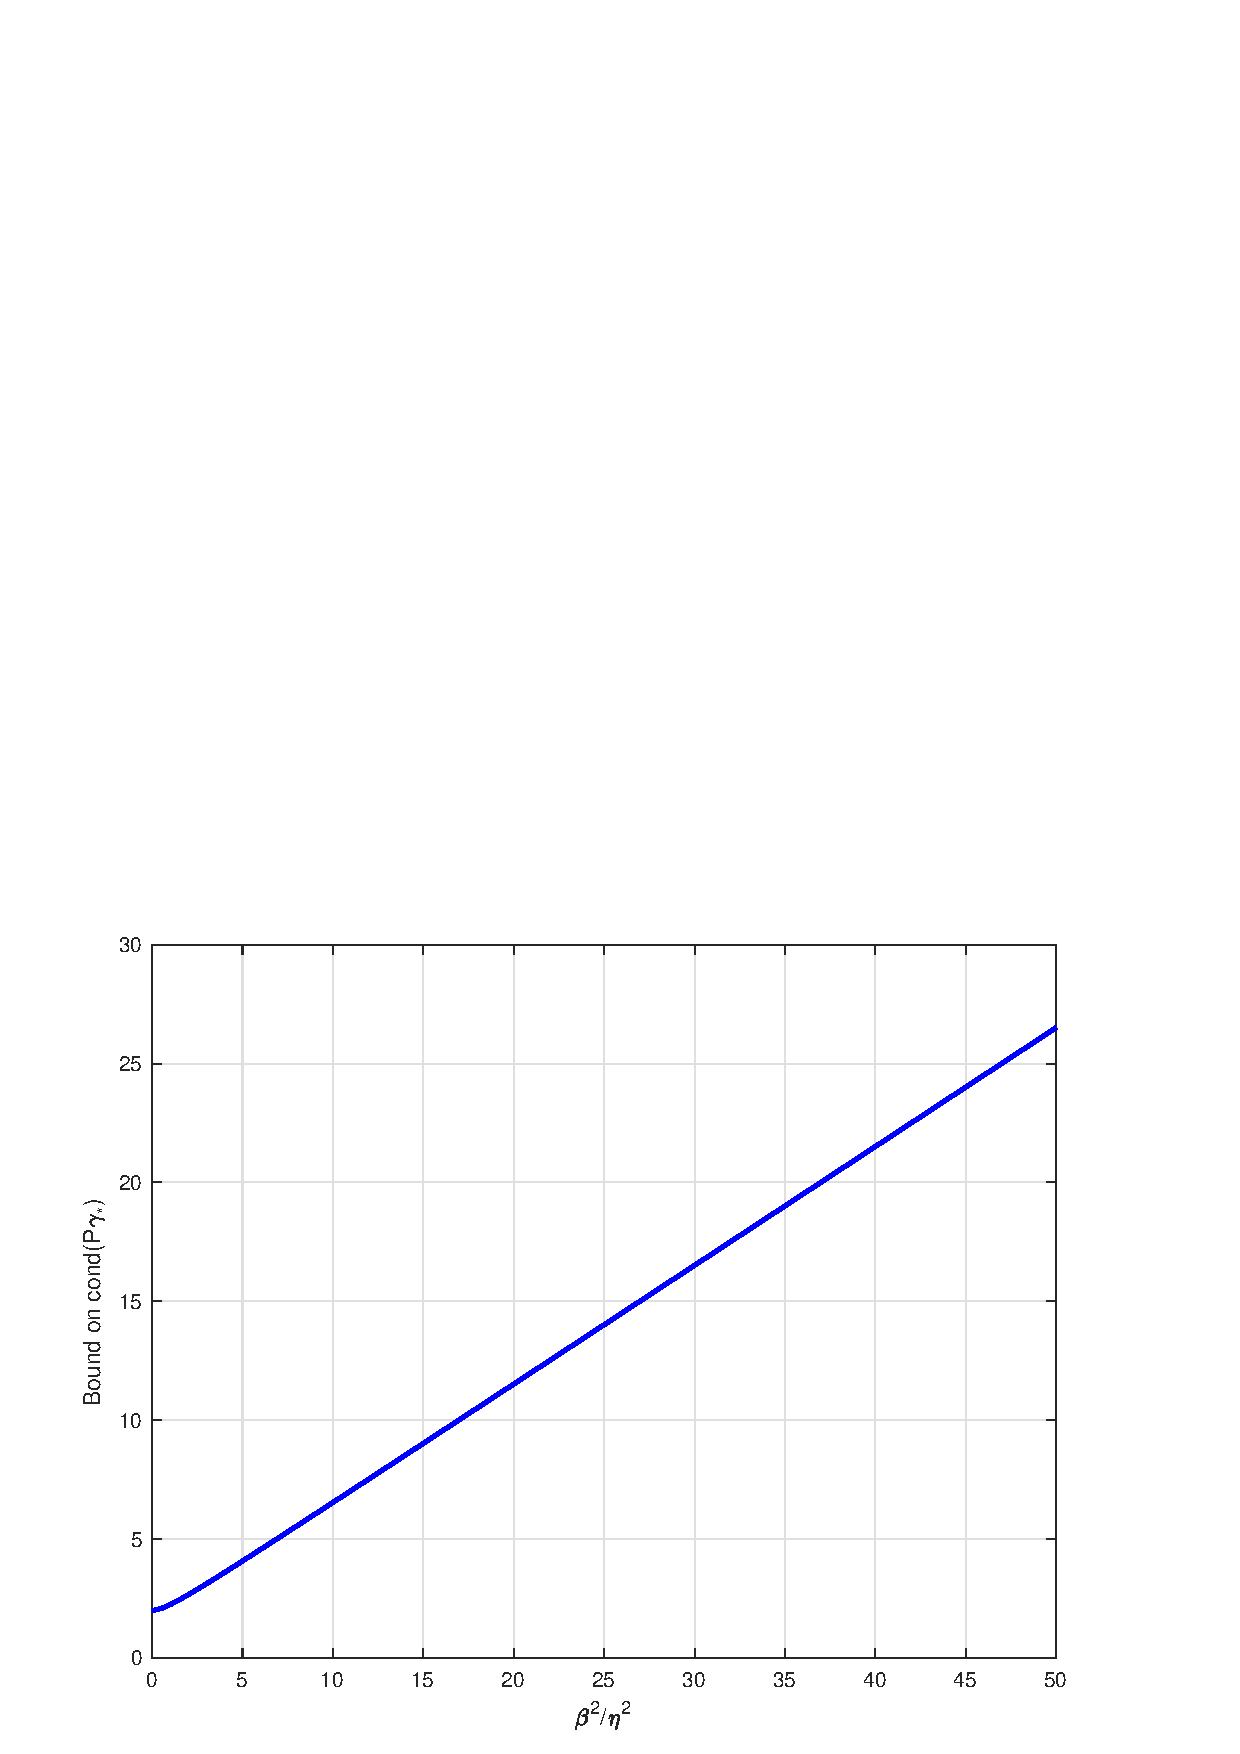
\includegraphics[width = 0.6\textwidth]{./cond.pdf}
\caption{Condition-number bounds from \Cref{th:cond} as a function of $\beta^2/\eta^2$.
For implicit Runge Kutta, such as Gauss methods, $\beta^2/\eta^2\sim\mathcal{O}(1)$ for
any reasonably number of $\mathcal{O}(1)$ stages. Not sure what this ratio will look
like for the Polynomial methods, so I plotted up to 50 to show conditioning is still
pretty good.}
\label{fig:bound}
\end{figure}



% \begin{comment}

% ------------------------------------------------------------------------------------- %
% ------------------------------------------------------------------------------------- %
% ------------------------------------------------------------------------------------- %
\section{PRESB preconditioning}
% See "Preconditioners for two-by-two block matrices with square blocks"
\tcb{Mistake w/ constants in this section, in process of redoing. $\eta$ should
be on $I$ term not $\mathcal{L}$}.


Another preconditioning we can consider is the PRESB approach, where we transform
\eqref{eq:2x2} to the form
%
\begin{align}
\begin{bmatrix} \eta I - \mathcal{L} & \beta I\\ \beta I & -(\eta I - \mathcal{L}) \end{bmatrix}
	\begin{bmatrix} \hat{\mathbf{x}}\\\hat{\mathbf{y}}\end{bmatrix} & =
	\begin{bmatrix} \mathbf{f}\\-\mathbf{g}\end{bmatrix}\label{eq:2x2_neg}
\end{align}
%
and consider preconditioners of the form
%
\begin{align*}
\mathcal{M} := \begin{bmatrix} (\eta + 2\beta)I - \mathcal{L} & \beta I
	\\ \beta I & -(\eta I - \mathcal{L}) \end{bmatrix}.
\end{align*}
%
Note that
%
\begin{align*}
\begin{bmatrix} (\eta+2\beta)I - \mathcal{L} & \beta I
	\\ \beta I & -(\eta I - \mathcal{L}) \end{bmatrix} & = 
	\begin{bmatrix} I & \mathbf{0} \\ I & -( (\eta+\beta)I - \mathcal{L}) \end{bmatrix}
	\begin{bmatrix} I & \beta I	\\ \mathbf{0} & I \end{bmatrix}
	\begin{bmatrix} (\eta+\beta)I - \mathcal{L} & \mathbf{0} \\ I & I \end{bmatrix} \\
& \hspace{-10ex} =
	\begin{bmatrix} I & \mathbf{0} \\ I & I \end{bmatrix}
	\begin{bmatrix} I & \mathbf{0} \\ \mathbf{0} & -( (\eta+\beta)I - \mathcal{L}) \end{bmatrix}
	\begin{bmatrix} I & \beta I	\\ \mathbf{0} & I \end{bmatrix}
	\begin{bmatrix} (\eta+\beta)I - \mathcal{L} & \mathbf{0} \\ \mathbf{0} & I \end{bmatrix}
	\begin{bmatrix} I & \mathbf{0} \\ I & I \end{bmatrix}.
\end{align*}
%
It follows that
%
\begin{align}\label{eq:presb_inv}
\mathcal{M}^{-1} & = 
	\begin{bmatrix} I & \mathbf{0} \\ -I & I \end{bmatrix}
	\begin{bmatrix} ((\eta+\beta)I - \mathcal{L})^{-1} & \mathbf{0} \\
		\mathbf{0} & I \end{bmatrix}
	\begin{bmatrix} I & -\beta I \\ \mathbf{0} & I \end{bmatrix}
	\begin{bmatrix} I & \mathbf{0} \\
		\mathbf{0} & -((\eta+\beta)I - \mathcal{L})^{-1} \end{bmatrix}
	\begin{bmatrix} I & \mathbf{0} \\ -I & I \end{bmatrix}.
\end{align}
%

Now consider the preconditioned operator $\mathcal{P} := \mathcal{M}^{-1}A$,
where $A$ is the system matrix in \eqref{eq:2x2_neg}. For compact notation,
the following equation will apply each block in $\mathcal{M}^{-1}$ \eqref{eq:presb_inv}
to $A$ \eqref{eq:2x2_neg} succcessively, where a $\mapsto$ sign indicates applying
the next block of $\mathcal{M}^{-1}$:
%
\begin{align*}
\begin{bmatrix} \eta I - \mathcal{L} & \beta I\\
	\beta I & -(\eta I - \mathcal{L}) \end{bmatrix} & \mapsto 
\begin{bmatrix} \eta I - \mathcal{L} & \beta I \\
	-( (\eta-\beta)I - \mathcal{L}) & -( (\eta+\beta)I - \mathcal{L}) \end{bmatrix} \\
& \mapsto \begin{bmatrix} \eta I - \mathcal{L} & \beta I \\
	((\eta+\beta)I - \mathcal{L})^{-1}( (\eta-\beta)I - \mathcal{L}) & I \end{bmatrix} \\
& \mapsto \begin{bmatrix} \eta I - \mathcal{L} -
		\beta((\eta+\beta)I - \mathcal{L})^{-1}( (\eta-\beta)I - \mathcal{L}) & \mathbf{0} \\
	((\eta+\beta)I - \mathcal{L})^{-1}( (\eta-\beta)I - \mathcal{L}) & I \end{bmatrix} \\
& = \begin{bmatrix} ((\eta+\beta)I - \mathcal{L}) -
		\beta[I + ((\eta+\beta)I - \mathcal{L})^{-1}((\eta-\beta)I - \mathcal{L})] & \mathbf{0} \\
	((\eta+\beta)I - \mathcal{L})^{-1}( (\eta-\beta)I - \mathcal{L}) & I \end{bmatrix} \\
& = \begin{bmatrix} ((\eta+\beta)I - \mathcal{L}) -
		2\beta((\eta+\beta)I - \mathcal{L})^{-1}(\eta I - \mathcal{L}) & \mathbf{0} \\
	((\eta+\beta)I - \mathcal{L})^{-1}( (\eta-\beta)I - \mathcal{L}) & I \end{bmatrix} \\
& \mapsto \begin{bmatrix} I -
		2\beta((\eta+\beta)I - \mathcal{L})^{-2}(\eta I - \mathcal{L}) & \mathbf{0} \\
	((\eta+\beta)I - \mathcal{L})^{-1}( (\eta-\beta)I - \mathcal{L}) & I \end{bmatrix} \\
& = \begin{bmatrix} I -
		2\beta((\eta+\beta)I - \mathcal{L})^{-2}(\eta I - \mathcal{L}) & \mathbf{0} \\
	((\eta+\beta)I - \mathcal{L})^{-2}( (\eta I - \mathcal{L})^2 - \beta^2I) & I \end{bmatrix} \\
& \mapsto \begin{bmatrix} I -
		2\beta((\eta+\beta)I - \mathcal{L})^{-2}(\eta I - \mathcal{L}) & \mathbf{0} \\
	((\eta+\beta)I - \mathcal{L})^{-2}( (\eta I - \mathcal{L})^2 + 2\beta(\eta I - \mathcal{L}) - \beta^2I) - I& I \end{bmatrix}.
\end{align*}
%
Note, by commutation of operators and their inverse we then have
%
\begin{align*}
\mathcal{P} & =  \begin{bmatrix} I -
		2\beta(\eta I - \mathcal{L})((\eta+\beta)I - \mathcal{L})^{-2} & \mathbf{0} \\
	( (\eta I - \mathcal{L})^2 + 2\beta(\eta I - \mathcal{L}) - \beta^2I)
		((\eta+\beta)I - \mathcal{L})^{-2} - I& I \end{bmatrix} \\
& = I - \begin{bmatrix} 2\beta(\eta I - \mathcal{L}) & \mathbf{0} \\ 
		((\eta+\beta)I - \mathcal{L})^{2} - ( (\eta I - \mathcal{L})^2 +
			2\beta(\eta I - \mathcal{L}) - \beta^2I) & \mathbf{0} \end{bmatrix}
		\begin{bmatrix} ((\eta+\beta)I - \mathcal{L})^{-2} & \mathbf{0} \\
		\mathbf{0} & I \end{bmatrix} \\
& = I - 2\beta\begin{bmatrix} (\eta I - \mathcal{L}) & \mathbf{0} \\ 
		\beta I & \mathbf{0} \end{bmatrix}
	\begin{bmatrix} ((\eta+\beta)I - \mathcal{L})^{-2} & \mathbf{0} \\
		\mathbf{0} & I \end{bmatrix}.
\end{align*}
%
Then, 
%
\begin{align*}
\min_{\mathbf{v}\neq\mathbf{0}} (\max_{\mathbf{v}\neq\mathbf{0}})
	\frac{\|\mathcal{P}\mathbf{v}\|^2}{\|\mathbf{v}\|^2}
& = \min_{[\mathbf{x},\mathbf{y}]\neq\mathbf{0}}
		(\max_{[\mathbf{x},\mathbf{y}]\neq\mathbf{0}})
	\frac{\left\|\left(I - 2\beta \begin{bmatrix} (\eta I - \mathcal{L}) & \mathbf{0} \\ 
		\beta I & \mathbf{0} \end{bmatrix}
	\begin{bmatrix} ((\eta +\beta)I - \mathcal{L})^{-2} & \mathbf{0} \\
		\mathbf{0} & I \end{bmatrix}\right)
		\begin{bmatrix} \mathbf{x}\\\mathbf{y}\end{bmatrix}\right\|^2}
		{\left\|\begin{bmatrix} \mathbf{x}\\\mathbf{y}\end{bmatrix}\right\|^2} \\
& = \min_{[\mathbf{x},\mathbf{y}]\neq\mathbf{0}}
		(\max_{[\mathbf{x},\mathbf{y}]\neq\mathbf{0}})
	\frac{\left\|\left(\begin{bmatrix} ((\eta +\beta)I - \mathcal{L})^{2} & \mathbf{0} \\
		\mathbf{0} & I \end{bmatrix}
		- 2\beta \begin{bmatrix} (\eta I - \mathcal{L}) & \mathbf{0} \\ 
		\beta I & \mathbf{0} \end{bmatrix}\right)
		\begin{bmatrix} \mathbf{x}\\\mathbf{y}\end{bmatrix}\right\|^2}
		{\left\|\begin{bmatrix} ((\eta +\beta)I - \mathcal{L})^{2}\mathbf{x}\\
			\mathbf{y}\end{bmatrix}\right\|^2} \\
& = \min_{[\mathbf{x},\mathbf{y}]\neq\mathbf{0}}
		(\max_{[\mathbf{x},\mathbf{y}]\neq\mathbf{0}})
	\frac{\left\|\begin{bmatrix} \beta^2 I + (\eta I - \mathcal{L})^{2} & \mathbf{0} \\
		- 2\beta^2 I & I \end{bmatrix}
		\begin{bmatrix} \mathbf{x}\\\mathbf{y}\end{bmatrix}\right\|^2}
		{\left\|\begin{bmatrix} ((\eta +\beta)I - \mathcal{L})^{2}\mathbf{x}\\
			\mathbf{y}\end{bmatrix}\right\|^2} \\
& = \min_{[\mathbf{x},\mathbf{y}]\neq\mathbf{0}}
		(\max_{[\mathbf{x},\mathbf{y}]\neq\mathbf{0}})
	\frac{\left\|(\beta^2I + (\eta I - \mathcal{L})^{2})\mathbf{x}\right\|^2 +
			\left\|\mathbf{y}\right\|^2
			+ 4\beta^4\|\mathbf{x}\|^2 - 4\beta^2\left\langle 
				\mathbf{y}, \mathbf{x}\right\rangle}
		{\left\|((\eta +\beta)I - \mathcal{L})^{2}\mathbf{x}\right\|^2 +
			\left\|\mathbf{y}\right\|^2}.
\end{align*}
%
\tcb{Below here might not be correct}

Note above that the $\|\mathbf{y}\|^2$ term simply adds a real scalar $\geq 0$
to the numerator and denominator. Since we are only interested in minimizing or
maximizing over $[\mathbf{x},\mathbf{y}]\neq\mathbf{0}$, we can limit $\mathbf{y}$
to be parallel to $\mathbf{x}$. To see this, let $\|\mathbf{y}\| = C$ and note
that when maximizing, $\|\mathbf{y}\|^2 -4\beta^2 \langle \mathbf{y},\mathbf{x} \rangle
\leq \|\mathbf{y}\|^2 + 4\beta^2\|\mathbf{y}\|\|\mathbf{x}\|
= C^2 + 4\beta^2C\|\mathbf{x}\|$, with equality at $\mathbf{y} := -C\mathbf{x}$.
Similar arguments apply for the minimum.\tcb{This might not be correct..}

Thus our problem can be reduced to a min/max over vector $\mathbf{x}\neq\mathbf{0}$
and scalar $C\in\mathbb{R}$:
\begin{align*}
\min_{\mathbf{v}\neq\mathbf{0}} (\max_{\mathbf{v}\neq\mathbf{0}})
	\frac{\|\mathcal{P}\mathbf{v}\|^2}{\|\mathbf{v}\|^2}
& = \min_{\mathbf{x}\neq\mathbf{0}, C\in\mathbb{R}}
		(\max_{\mathbf{x}\neq\mathbf{0}, C\in\mathbb{R}})
	\frac{\left\|(\beta^2I + (I - \eta\mathcal{L})^{2})\mathbf{x}\right\|^2 +
			C^2\left\|\mathbf{x}\right\|^2
			+ 4\beta^4\|\mathbf{x}\|^2 - 4C\beta^2\|\mathbf{x}\|^2}
		{\left\|((1+\beta)I - \eta\mathcal{L})^{2}\mathbf{x}\right\|^2 +
			C^2\left\|\mathbf{x}\right\|^2} \\
& = \min_{\mathbf{x}\neq\mathbf{0}, C\in\mathbb{R}}
		(\max_{\mathbf{x}\neq\mathbf{0}, C\in\mathbb{R}})
	\frac{\left\|(\beta^2I + (I - \eta\mathcal{L})^{2})\mathbf{x}\right\|^2 +
			(2\beta^2 - C)^2\left\|\mathbf{x}\right\|^2}
		{\left\|((1+\beta)I - \eta\mathcal{L})^{2}\mathbf{x}\right\|^2 +
			C^2\left\|\mathbf{x}\right\|^2} .
\end{align*}
%
By the assumption that $W(\mathcal{L}) \leq 0$, for real-valued $\mathbf{x}$ we have
%
\begin{align*}
\left\|(\eta I - \mathcal{L})\mathbf{x}\right\|^2 & =
	\eta^2\|\mathbf{x}\|^2 - 2\eta\langle \mathcal{L}\mathbf{x},\mathbf{x}\rangle +
		\|\mathcal{L}\mathbf{x}\|^2
\geq \eta^2\|\mathbf{x}\|^2 + \|\mathcal{L}\mathbf{x}\|^2 \geq \eta^2\|\mathbf{x}\|^2.
\end{align*}
%
Then consider the denominator term, 
%
\begin{align*}
\left\|((\eta+\beta)I - \mathcal{L})^{2}\mathbf{x}\right\|^2
	& = \left\| [( \beta^2I + (\eta I - \mathcal{L})^{2}) + 2\beta(\eta I - \mathcal{L})]
		\mathbf{x}\right\|^2 \\
& = \left\| ( \beta^2I + (\eta I - \mathcal{L})^{2})\mathbf{x}\right\|^2 +
	4\beta^2\left\|(\eta I - \mathcal{L})\mathbf{x}\right\|^2 +
	8\beta^2 \left\langle ( \beta^2I + (\eta I - \mathcal{L})^{2})\mathbf{x},
		 (\eta I - \mathcal{L})\mathbf{x}\right\rangle \\
& = \left\| ( \beta^2I + (\eta I - \mathcal{L})^{2})\mathbf{x}\right\|^2 +
	4\beta^2\left\|(\eta I - \mathcal{L})\mathbf{x}\right\|^2 +
	8\beta^4 \left\langle \mathbf{x}, (\eta I - \mathcal{L})\mathbf{x}\right\rangle + 
	\\&\hspace{10ex}
	8\beta^2 \left\langle (\eta I - \mathcal{L})[ (\eta I - \mathcal{L})\mathbf{x}] ,
		 (\eta I - \mathcal{L})\mathbf{x}\right\rangle \\
& = \left\| ( \beta^2I + (\eta I - \mathcal{L})^{2})\mathbf{x}\right\|^2 +
	4\beta^2\left\|(\eta I - \mathcal{L})\mathbf{x}\right\|^2 +
	8\beta^4\|\mathbf{x}\|^2 - 
	\\&\hspace{10ex}
	8\eta\beta^4 \left\langle \mathbf{x}, \mathcal{L}\mathbf{x}\right\rangle + 
	8\beta^2 \left\|(\eta I - \mathcal{L})\mathbf{x}\right\|^2 -
	8\eta\beta^2\left\langle \mathcal{L}(\eta I - \mathcal{L})\mathbf{x} ,
		 (\eta I - \mathcal{L})\mathbf{x}\right\rangle, \\
& = \left\| ( \beta^2I + (\eta I - \mathcal{L})^{2})\mathbf{x}\right\|^2 +
	12\beta^2\left\|(\eta I - \mathcal{L})\mathbf{x}\right\|^2 +
	8\beta^4\|\mathbf{x}\|^2 - 
	\\&\hspace{10ex}
	8\eta\beta^4 \left\langle \mathbf{x}, \mathcal{L}\mathbf{x}\right\rangle -
	8\eta\beta^2\left\langle \mathcal{L}(\eta I - \mathcal{L})\mathbf{x} ,
		 (\eta I - \mathcal{L})\mathbf{x}\right\rangle, \\
& \geq \left\| ( \beta^2I + (\eta I - \mathcal{L})^{2})\mathbf{x}\right\|^2 +
	12\beta^2\left\|(\eta I - \mathcal{L})\mathbf{x}\right\|^2 +
	8\beta^4\|\mathbf{x}\|^2 \\
& \geq \left\| ( \beta^2I + (\eta I - \mathcal{L})^{2})\mathbf{x}\right\|^2 +
	(8\beta^4 + 12\beta^2)\|\mathbf{x}\|^2.
\end{align*}
% 
Considering the minimum, we then have
\begin{align*}
\min_{\mathbf{v}\neq\mathbf{0}}	\frac{\|\mathcal{P}\mathbf{v}\|^2}{\|\mathbf{v}\|^2}
	& \leq \min_{\mathbf{x}\neq\mathbf{0}, C\in\mathbb{R}}
	\frac{\left\|(\beta^2I + (I - \mathcal{L})^{2})\mathbf{x}\right\|^2 +
			(2\beta^2 - C)^2\left\|\mathbf{x}\right\|^2}
		{\left\| ( \beta^2I + (I - \eta\mathcal{L})^{2})\mathbf{x}\right\|^2 +
	(8\beta^4 + 12\beta^2 + C^2)\|\mathbf{x}\|^2}
\end{align*}
%
\tcb{
Overall this does not seem good. If we let $C = 2\beta^2$...}


% ------------------------------------------------------------------------------------- %
% ------------------------------------------------------------------------------------- %
\subsection{Skew-symmetric operators}

The above preconditioning is known to work well for SPD operators, but the above
analysis suggests otherwise in general. Thus consider skew symmetric operators.
Let $U$ denote the eigenvector matrix for $\mathcal{L} = UDU^*$, where
$UU^* = U^*U = I$ and $D$ is diagonal and purely imaginary. 


Then 
%
\begin{align*}
\begin{bmatrix} U^* & \mathbf{0} \\ \mathbf{0} & U^*\end{bmatrix}
	\mathcal{P}\begin{bmatrix} U & \mathbf{0} \\ \mathbf{0} & U\end{bmatrix} & =
I - 2\beta\begin{bmatrix} U^* & \mathbf{0} \\ \mathbf{0} & U^*\end{bmatrix}
	\begin{bmatrix} (I - \eta\mathcal{L}) & \mathbf{0} \\ 
	\beta I & \mathbf{0} \end{bmatrix}
	\begin{bmatrix} ((1+\beta)I - \eta\mathcal{L})^{-2} & \mathbf{0} \\
		\mathbf{0} & I \end{bmatrix}
	\begin{bmatrix} U & \mathbf{0} \\ \mathbf{0} & U\end{bmatrix} \\
& = I - 2\beta \begin{bmatrix} (I - \eta D) & \mathbf{0} \\ 
	\beta I & \mathbf{0} \end{bmatrix}
	\begin{bmatrix} ((1+\beta)I - \eta D)^{-2} & \mathbf{0} \\
		\mathbf{0} & I \end{bmatrix} \\
& = \begin{bmatrix} I - 2\beta(I - \eta D)((1+\beta)I - \eta D)^{-2} & \mathbf{0} \\ 
	-2\beta^2 ((1+\beta)I - \eta D)^{-2} & I \end{bmatrix} \\
& := \begin{bmatrix} I - 2\beta D_1D_2^{-2} & \mathbf{0} \\ -2\beta^2D_2^{-2} & I \end{bmatrix},
\end{align*}
%
where $D_1 := (I - \eta D)$ and $D_2 := ((1+\beta)I - \eta D)^{-2}$ are
complex diagonal matrices. Then the minimum and maximum singular values are
given by the square root of the minimum and maximum eigenvalue of $A^*A$
of the above equations. Since each of the $2\times 2$ block matrices are
diagonal, we have
%
\begin{align*}
\begin{bmatrix} I - 2\beta D_1D_2^{-2} & \mathbf{0} \\ -2\beta^2D_2^{-2} & I \end{bmatrix}
	\begin{bmatrix} I - 2\beta D_1D_2^{-2} & \mathbf{0} \\ -2\beta^2D_2^{-2} & I \end{bmatrix}^*
& = \begin{bmatrix} I - 2\beta D_1D_2^{-2} & \mathbf{0} \\ -2\beta^2D_2^{-2} & I \end{bmatrix}
	\begin{bmatrix} I - 2\beta \overline{D_1D_2^{-2}} & -2\beta^2\overline{D_2^{-2}}\\ \mathbf{0} & I \end{bmatrix} \\
& = \begin{bmatrix}  (I - 2\beta D_1D_2^{-2})( I - 2\beta\overline{D_1D_2^{-2}}) & -2\beta^2\overline{D_2^{-2}}
	(I - 2\beta D_1D_2^{-2}) \\ -2\beta^2D_2^{-2}( I - 2\beta \overline{D_1D_2^{-2}}) &
		I + 4\beta^4 D_2^{-2}\overline{D_2^{-2}} \end{bmatrix}.
\end{align*}
%
This looks complicated, but note that a $2\times 2$ block matrix where each
block is a diagonal matrix can be unitarily permuted to be a block-diagonal
matrix with $2\times 2$ (scalar) diagonal blocks. The eigenvalues of the
larger operator are then given by the eigenvalues of these individual $2\times 2$
complex matrices. Let $\mathrm{i}\zeta$ denote an eigenvalue of $\mathcal{L}$. Then,
the corresponding elements of the block-diagonal matrices take the form
%
\begin{align*}
(I - 2\beta D_1D_2^{-2})( I - 2\beta\overline{D_1D_2^{-2}}) & \mapsto 
	\left( 1 - 2\beta \frac{1 - \mathrm{i}\eta\zeta}{(1+\beta - \mathrm{i}\eta\zeta)^{2}}\right)
		\left(1 - 2\beta\frac{1 + \mathrm{i}\eta\zeta}{(1+\beta + \mathrm{i}\eta\zeta)^{2}}\right)
\end{align*}


% \end{comment}

% ------------------------------------------------------------------------------------- %
% ------------------------------------------------------------------------------------- %
% ------------------------------------------------------------------------------------- %
\section{One-constant block preconditioner}

Consider preconditioners for \eqref{eq:2x2} of the form
%
\begin{align*}
\mathcal{M} := \begin{bmatrix} \gamma I - \mathcal{L} & \mathbf{0} \\
	-\beta I & I - \gamma\mathcal{L}) \end{bmatrix}
\end{align*}
%
The left preconditioned operator is given by
%
\begin{align*}
\mathcal{P}_\gamma :&= \begin{bmatrix} \gamma I - \mathcal{L} & \mathbf{0} \\
		-\beta I & \gamma I - \mathcal{L} \end{bmatrix}^{-1}
	\begin{bmatrix} \eta I - \mathcal{L} & \beta I \\
	-\beta I & \eta I - \mathcal{L} \end{bmatrix} \\
& = \begin{bmatrix} (\gamma I - \mathcal{L})^{-1} & \mathbf{0} \\
		\beta (\gamma I - \mathcal{L})^{-2} & (\gamma I - \mathcal{L})^{-1} \end{bmatrix}
	\begin{bmatrix} \eta I - \mathcal{L} & \beta I \\
	-\beta I & \eta I - \mathcal{L} \end{bmatrix} \\
& = \begin{bmatrix} I - (\gamma -\eta )(\gamma I - \mathcal{L})^{-1} & 
		\beta (\gamma I - \mathcal{L})^{-1} \\
		-\beta (\gamma -\eta )(\gamma I - \mathcal{L})^{-2} & 
		I - (\gamma -\eta )(\gamma I - \mathcal{L})^{-1} +
			\beta^2(\gamma I - \mathcal{L})^{-2}
	\end{bmatrix}.
\end{align*}
%
The right-preconditioned operator is given by
%
\begin{align*}
\mathcal{P}_\gamma^R :&= \begin{bmatrix} \eta I - \mathcal{L} & \beta I \\
	-\beta I & \eta I - \mathcal{L} \end{bmatrix}
	\begin{bmatrix} \gamma I - \mathcal{L} & \mathbf{0} \\
		-\beta I & \gamma I - \mathcal{L} \end{bmatrix}^{-1} \\
& = \begin{bmatrix} \eta I - \mathcal{L} & \beta I \\
	-\beta I & \eta I - \mathcal{L} \end{bmatrix}
	\begin{bmatrix} (\gamma I - \mathcal{L})^{-1} & \mathbf{0} \\
		\beta (\gamma I - \mathcal{L})^{-2} & (\gamma I - \mathcal{L})^{-1} \end{bmatrix}\\
& = \begin{bmatrix} I - (\gamma -\eta )(\gamma I - \mathcal{L})^{-1} +
			\beta^2(\gamma I - \mathcal{L})^{-2} & 
		\beta (\gamma I - \mathcal{L})^{-1} \\
		-\beta (\gamma -\eta )(\gamma I - \mathcal{L})^{-2} & 
		I - (\gamma -\eta )(\gamma I - \mathcal{L})^{-1}
	\end{bmatrix} \\
\end{align*}


%
Now consider the max/min singular values of the right-preconditioned operator,
%
\begin{align*}
&\hspace{-5ex} \min_{\mathbf{v}\neq\mathbf{0}} (\max_{\mathbf{v}\neq\mathbf{0}})
	\frac{\|\mathcal{P}_\gamma^R\mathbf{v}\|^2}{\|\mathbf{v}\|^2} \\
& = \min_{[\mathbf{x},\mathbf{y}]\neq\mathbf{0}} (\max_{[\mathbf{x},\mathbf{y}]\neq\mathbf{0}})
	\frac{ \left\| \begin{bmatrix} I - (\gamma -\eta )(\gamma I - \mathcal{L})^{-1} +
			\beta^2(\gamma I - \mathcal{L})^{-2} & 
		\beta (\gamma I - \mathcal{L})^{-1} \\
		-\beta (\gamma -\eta )(\gamma I - \mathcal{L})^{-2} & 
		I - (\gamma -\eta )(\gamma I - \mathcal{L})^{-1}
	\end{bmatrix}
	\begin{bmatrix} \mathbf{x} \\ \mathbf{y}\end{bmatrix} \right\|^2}
	{ \left\| \begin{bmatrix} \mathbf{x} \\ \mathbf{y}\end{bmatrix} \right\|^2} \\
& = \min_{[\mathbf{x},\mathbf{y}]\neq\mathbf{0}} (\max_{[\mathbf{x},\mathbf{y}]\neq\mathbf{0}})
	\frac{ \left\| \begin{bmatrix} (\gamma I - \mathcal{L})^2 -
		(\gamma -\eta )(\gamma I - \mathcal{L}) +
			\beta^2 I & 
		\beta I  \\
		-\beta (\gamma -\eta ) I & 
		(\gamma I - \mathcal{L}) - (\gamma -\eta )I
	\end{bmatrix}
	\begin{bmatrix} \mathbf{x} \\ \mathbf{y}\end{bmatrix} \right\|^2}
	{ \left\| \begin{bmatrix} (\gamma I - \mathcal{L})^2 \mathbf{x} \\
		(\gamma I - \mathcal{L}) \mathbf{y}\end{bmatrix} \right\|^2} \\
& = \min_{[\mathbf{x},\mathbf{y}]\neq\mathbf{0}} (\max_{[\mathbf{x},\mathbf{y}]\neq\mathbf{0}})
	\frac{ \left\| \begin{bmatrix} (\beta^2+\eta\gamma)I - (\gamma+\eta)\mathcal{L} + \mathcal{L}^2& 
		\beta I  \\ -\beta (\gamma -\eta ) I & \eta I - \mathcal{L}
	\end{bmatrix}
	\begin{bmatrix} \mathbf{x} \\ \mathbf{y}\end{bmatrix} \right\|^2}
	{ \left\| \begin{bmatrix} (\gamma^2 I - 2 \gamma\mathcal{L} + \mathcal{L}^2) \mathbf{x} \\
		(\gamma I - \mathcal{L}) \mathbf{y}\end{bmatrix} \right\|^2} \\
\end{align*}
%
We could make the strategic choice $\gamma = \frac{\eta + \sqrt{\eta^2+4\beta^2}}{2}$
such that $\beta^2 = \gamma(\gamma-\eta)$. This eliminates the identity term, which
yields
%
\begin{align*}
&\hspace{-5ex} \min_{\mathbf{v}\neq\mathbf{0}} (\max_{\mathbf{v}\neq\mathbf{0}})
	\frac{\|\mathcal{P}_\gamma^R\mathbf{v}\|^2}{\|\mathbf{v}\|^2} \\
& = \min_{[\mathbf{x},\mathbf{y}]\neq\mathbf{0}} (\max_{[\mathbf{x},\mathbf{y}]\neq\mathbf{0}})
	\frac{ \left\| \begin{bmatrix} (\gamma I - \mathcal{L})^2 + (\gamma -\eta )\mathcal{L} & 
		\beta I  \\ -\beta (\gamma -\eta ) I & 
		(\gamma I - \mathcal{L}) - (\gamma -\eta )I
	\end{bmatrix}
	\begin{bmatrix} \mathbf{x} \\ \mathbf{y}\end{bmatrix} \right\|^2}
	{ \left\| \begin{bmatrix} (\gamma I - \mathcal{L})^2 \mathbf{x} \\
		(\gamma I - \mathcal{L}) \mathbf{y}\end{bmatrix} \right\|^2} \\
& = \min_{[\mathbf{x},\mathbf{y}]\neq\mathbf{0}} (\max_{[\mathbf{x},\mathbf{y}]\neq\mathbf{0}})
	\frac{ \left\| \begin{bmatrix} (\gamma I - \mathcal{L}) +
			(\gamma -\eta )\mathcal{L}(\gamma I - \mathcal{L})^{-1} & 
		\beta I  \\ -\beta (\gamma -\eta ) (\gamma I - \mathcal{L})^{-1} & 
		(\gamma I - \mathcal{L}) - (\gamma -\eta )I
	\end{bmatrix}
	\begin{bmatrix} \mathbf{x} \\ \mathbf{y}\end{bmatrix} \right\|^2}
	{ \left\| \begin{bmatrix} (\gamma I - \mathcal{L}) \mathbf{x} \\
		(\gamma I - \mathcal{L}) \mathbf{y}\end{bmatrix} \right\|^2} \\
& = \min_{[\mathbf{x},\mathbf{y}]\neq\mathbf{0}} (\max_{[\mathbf{x},\mathbf{y}]\neq\mathbf{0}})
	\frac{ \left\| \begin{bmatrix} (\gamma I - \mathcal{L}) -
			(\gamma -\eta )(I - \gamma \mathcal{L}^{-1})^{-1} & 
		\beta I  \\ -\beta (\gamma -\eta ) (\gamma I - \mathcal{L})^{-1} & 
		(\gamma I - \mathcal{L}) - (\gamma -\eta )I
	\end{bmatrix}
	\begin{bmatrix} \mathbf{x} \\ \mathbf{y}\end{bmatrix} \right\|^2}
	{ \left\| \begin{bmatrix} (\gamma I - \mathcal{L}) \mathbf{x} \\
		(\gamma I - \mathcal{L}) \mathbf{y}\end{bmatrix} \right\|^2} \\
& = \min_{[\mathbf{x},\mathbf{y}]\neq\mathbf{0}} (\max_{[\mathbf{x},\mathbf{y}]\neq\mathbf{0}})
	\frac{ \left\| \begin{bmatrix} I -
			(\gamma -\eta )(I - \gamma \mathcal{L}^{-1})^{-1}(\gamma I - \mathcal{L})^{-1} & 
		\beta (\gamma I - \mathcal{L})^{-2}  \\ -\beta (\gamma -\eta ) (\gamma I - \mathcal{L})^{-1} & 
		I - (\gamma -\eta )(\gamma I - \mathcal{L})^{-1}
	\end{bmatrix}
	\begin{bmatrix} \mathbf{x} \\ \mathbf{y}\end{bmatrix} \right\|^2}
	{ \left\| \begin{bmatrix}  \mathbf{x} \\
		\mathbf{y}\end{bmatrix} \right\|^2} \\
\end{align*}


% ------------------------------------------------------------------------------------- %
% ------------------------------------------------------------------------------------- %
\bibliographystyle{plain}
\bibliography{refs2.bib}

\end{document}
















